\documentclass[tikz,border=12pt]{standalone}
\usepackage[T1]{fontenc}
\usepackage{helvet}
\renewcommand{\familydefault}{\sfdefault}
\usetikzlibrary{shapes.geometric,arrows.meta,positioning,fit,backgrounds,calc}

\definecolor{ink}{HTML}{2E3440}
\definecolor{svc}{HTML}{DCE6F2}    \definecolor{svcline}{HTML}{4C6A92}
\definecolor{store}{HTML}{E5EFE1}  \definecolor{storeline}{HTML}{5B8C5A}
\definecolor{ext}{HTML}{F3E9DC}    \definecolor{extline}{HTML}{A8763E}
\definecolor{async}{HTML}{6C757D}  \definecolor{alert}{HTML}{C0392B}
\definecolor{regionfill}{HTML}{F7F9FC}

\begin{document}
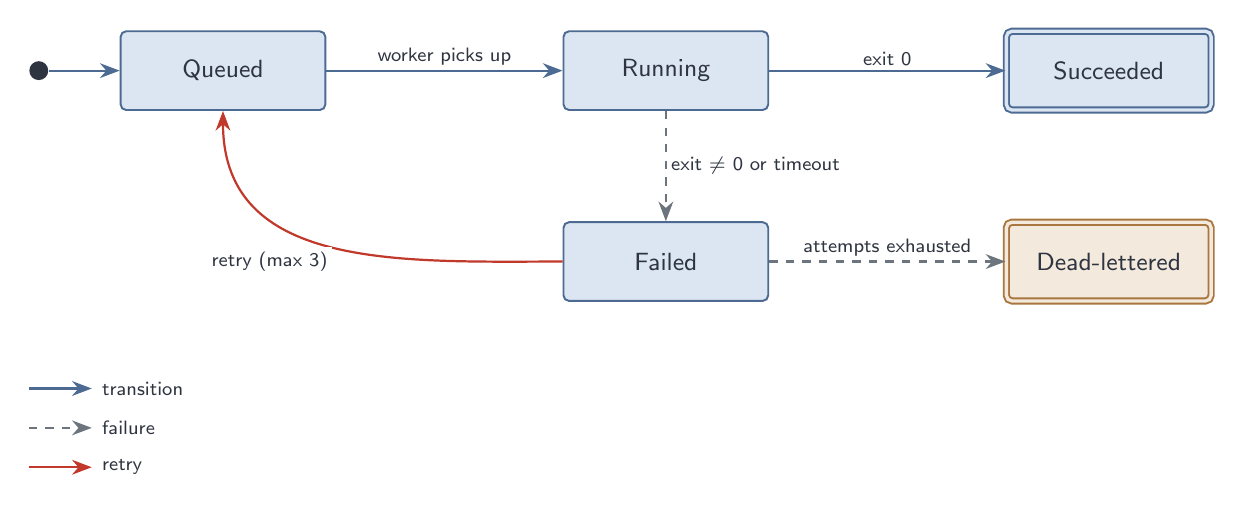
\begin{tikzpicture}[
  font=\small, color=ink, node distance=14mm and 30mm,
  box/.style={draw=svcline, fill=svc, rounded corners=2pt, minimum width=26mm,
              minimum height=10mm, align=center, line width=0.7pt},
  extbox/.style={box, draw=extline, fill=ext},
  terminal/.style={double, double distance=1.2pt},
  sync/.style={-{Stealth[length=2.5mm]}, line width=0.8pt, color=svcline},
  fail/.style={sync, dashed, color=async},
  retry/.style={sync, color=alert},
  lbl/.style={font=\scriptsize, fill=white, inner sep=1.5pt, text=ink},
]
% states
\node[box] (queued) {Queued};
\node[box, right=of queued] (running) {Running};
\node[box, terminal, double=svc, right=of running] (succeeded) {Succeeded};
\node[box, below=of running] (failed) {Failed};
\node[extbox, terminal, double=ext, right=of failed] (dead) {Dead-lettered};

% initial marker
\node[circle, fill=ink, inner sep=0pt, minimum size=2.4mm, left=9mm of queued] (init) {};
\draw[sync] (init) -- (queued);

% transitions
\draw[sync] (queued) -- (running) node[lbl, midway, above] {worker picks up};
\draw[sync] (running) -- (succeeded) node[lbl, midway, above] {exit 0};
\draw[fail] (running) -- (failed) node[lbl, midway, right] {exit $\neq$ 0 or timeout};
\draw[fail] (failed) -- (dead) node[lbl, midway, above] {attempts exhausted};
\draw[retry] (failed.west) to[out=180, in=-90, looseness=1.1]
  node[lbl, pos=0.5, anchor=north east] {retry (max 3)} (queued.south);

% legend
\begin{scope}[shift={($(init.west |- failed.south)+(0,-11mm)$)}, font=\scriptsize]
  \draw[sync]  (0,0)     -- ++(8mm,0) node[right, text=ink] {transition};
  \draw[fail]  (0,-5mm)  -- ++(8mm,0) node[right, text=ink] {failure};
  \draw[retry] (0,-10mm) -- ++(8mm,0) node[right, text=ink] {retry};
\end{scope}
\end{tikzpicture}
\end{document}
